\documentclass[11pt]{article}
\usepackage{fullpage}
\usepackage{graphics,epsfig,color}
\usepackage{wrapfig}
\usepackage{times}
\usepackage{setspace}
\usepackage{amsmath,amsthm,amssymb}
\usepackage{url}
\usepackage{fancyhdr}
\usepackage{enumitem}
\usepackage{graphvizzz}
\pagestyle{fancy}


\newtheorem{theorem}{Theorem}[section]
\newtheorem{corollary}{Corollary}[section]
\newtheorem{lemma}{Lemma}[section]
\newtheorem{problem}{Problem}
\newtheorem{definition}{Definition}[section]
\newtheorem{observation}{Observation}[section]
\newtheorem{example}{Example}[section]
\newtheorem{openproblem}{Open Problem}[section]
\newtheorem{fact}{Fact}[section]

\newcommand{\qedsymb}{\hfill{\rule{2mm}{2mm}}}
\newenvironment{proofsketch}
{
	\begin{trivlist}
	\item[\hspace{\labelsep}{\noindent Proof Sketch: }]
}{\qedsymb\end{trivlist}}



%the following few lines until usepackage{algorithm2e} is to avoid the
%conflicts of algorithm2e with other packages.
\makeatletter
\newif\if@restonecol
\makeatother
\let\algorithm\relax
\let\endalgorithm\relax
\usepackage[ruled,vlined,linesnumbered]{algorithm2e}

\newcommand{\remove}[1]{}



%--------------------------------


\begin{document}

	\renewcommand{\headrulewidth}{0.4pt}
	\setlength{\headheight}{38.0pt}
	\fancyhead[L]{\bf CSCD359 Homework1, Winter 2012, 
	Eastern Washington University. Cheney, Washington. \\
	\bigskip Name: Eric Fode\hspace{40mm}EWU ID:00530214}


	\noindent{\bf Solution for Problem 1}\\
	\noindent{\bf Idea:} Go through the list checking to see if the next item is less then the current node, if it is add it to the left
	then call this function on the new left node save the return value of this recursive call to be used as the index at which
	the right node gets added from, then call the function on the right node finally return the current position in the array.\\
	\begin{algorithm}[H]
				\NoCaptionOfAlgo
				\caption{\bf preOrderTree($treeArray,root,index$)}
				\KwIn{A preordered array,The root of the tree (starting with a node that has the first value of the array,the arrayIndex}
				\KwResult{The tree that the preorder array represent in attached to the root node}
				\Begin{
						\If{$treeArray[index] < root.value$}
						{
							$root.left = node(treeArray[index]))$\;
							$index \longleftarrow preOrderTree(treeArray,root.left,index)$\;
							$root.right = node(treeArray[index]))$\;
							$index \longleftarrow preOrderTree(treeArray,root.right,index)$\;
						}
						\Return $index+1$\;
						
						}				
			\end{algorithm}	
	\noindent{\bf Analysis:} This should take $O(n)$ time
		\bigskip
	
	\noindent{\bf Solution for Problem  2}\\
	\noindent{\bf Idea:} Find the mid point of the array make it the root of the current tree, recurse for the left and right sides of the tree
	using only the upper half or the lower half of the array until there are no items left
	
	\begin{algorithm}[H]
		\NoCaptionOfAlgo
		\caption{\bf sortedTree($treeArray$)}
		\KwIn{A slice of a sorted array}
		\KwResult{A BST that has a height bounded by $log(n)$}
		\Begin{
		
			\If{treeArray.size = 1}
			{
				\Return $new node(treeArray[0])$\;
			}
			$root = new node(treeArray[treeArray.size/2])$\;
			$root.left \longleftarrow sortedTree(treeArray[0:treeArray.size/2])$\;
			$root.right \longleftarrow sortedTree(treeArray[treeArray.size/2+1:treeArray.size])$\;
			\Return $root$\;
		}
		\end{algorithm}
	\noindent{\bf Analysis:} This should take $O(n)$ time
	\bigskip
	
	\noindent{\bf Solution for Problem 3}\\
	12 \\

\includegraphics{step1.pdf}\\
\includegraphics{step2.pdf}\\
	19 \\
	
\includegraphics{step3.pdf}\\
	17\\

\includegraphics{step4.pdf}\\

\includegraphics{step5.pdf}\\

\includegraphics{step6.pdf}\\
	21\\
\includegraphics{step7.pdf}\\

\includegraphics{step8.pdf}\\
	16\\
	
\includegraphics{step9.pdf}\\
	15\\
	
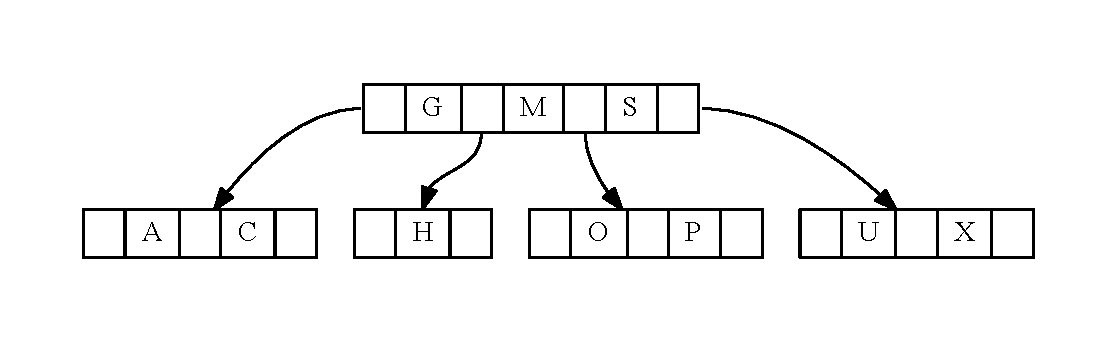
\includegraphics{step10.pdf}\\
	
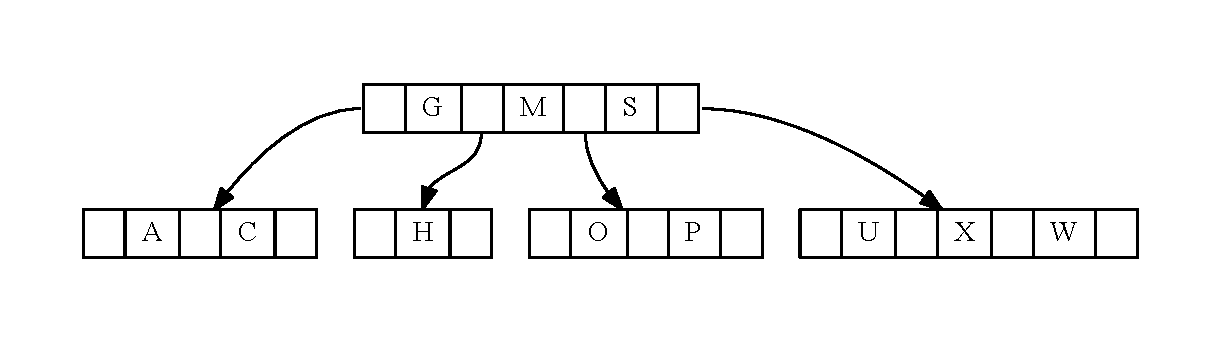
\includegraphics{step11.pdf}\\
\includegraphics{step12.pdf}
	\bigskip
	
	\noindent{\bf Solution for Problem 4}\\
	
\includegraphics{bstep0.pdf}\\
	14\\
\includegraphics{bstep1.pdf}\\
	1\\
\includegraphics{bstep2.pdf}\\
	5\\
\includegraphics{bstep3.pdf}\\
 2\\
\includegraphics{bstep4.pdf}\\
 11\\
\includegraphics{bstep5.pdf}\\
The rest of the step are basic bst pruning and do not need to be shown becuase they don't use any
of the Red-Black rules
\end{document}